\documentclass[11pt,fleqn,a4paper,]{LegrandOrangeBook}
\addbibresource{sample.bib} % Bibliography file
\definecolor{ocre}{RGB}{243, 102, 25} 
\chapterimage{orange1.jpg} 
\chapterspaceabove{6.5cm}
\chapterspacebelow{6.75cm} 
%\begin{theorem}[Name of the theorem]
%\begin{exercise}
%\begin{example}[Example name]
%\begin{definition}[Definition name]
%\begin{corollary}[Corollary name]
%\begin{remark}
%\begin{proposition}[Proposition name]
%\begin{problem}
%\begin{vocabulary}[Word]
%----------------------------------------------------------------------------------------
\begin{document}
%----------------------------------------------------------------------------------------
\section{CORRIENTES DE CONVECCIÓN Y CONDUCCIÓN}
\begin{definition}[Corriente]
La corriente (en amperios) a través de un área dada es la carga eléctrica que pasa por el área por unidad de tiempo.\\
\begin{equation}
\label{eq:corriente}
I=\frac{dQ}{dt}
\end{equation}
Donde\\
\begin{itemize}
\item Q:Carga(Coulomb)
\item t: Tiempo(Segundos)
\end{itemize}
Así, en una corriente de un amperio, la carga se transfiere a razón de un culombio por segundo.
\end{definition}
\begin{definition}[Densidad de corriente eléctrica]
Ahora presentamos el concepto de densidad de corriente J. Si la corriente $\delta$I fluye a través de un plano superficie $\delta$S, la densidad de corriente es:
\begin{equation}
\label{eq: densidad de corriente}
J=\frac{\delta I}{\delta S}
\end{equation}
Donde:
\begin{itemize}
\item I: Intensidad de corriente(Coulomb).
\item S: Superficie($m^2$).
\end{itemize}
\end{definition}
Se puede deducir la Intensidad de corriente en términos de la Densidad de corriente como:
\begin{equation}
\label{eq:intensidad y densidad de corriente}
I=\int_SJ\cdot dS
\end{equation}
Se presenta una ecuación más representativas de la corriente de conducción\footnote{Existen formas alternativas, estas pueden ser encontradas en el libro \cite{sadiku2018elements}}.
\begin{equation}\label{eq:JsigmaE}
J=\sigma E
\end{equation}
Donde:
\begin{itemize}
\item $\sigma$: Conductividad del conductor
\end{itemize}
\section{Conductores}
Un conductor tiene una gran cantidad de carga que puede moverse libremente. Consideraremos dos casos involucrando a un conductor.
\subsection{Conductor Isolado}
Un conductor perfecto($\sigma=\infty$) no puede un campo electrostático en el, por lo tanto dentro del conductor:
\begin{displaymath}
E=0, \rho_v=0, V_{ab}=0
\end{displaymath}
Donde:
\begin{itemize}
\item E: Campo eléctrico.
\item $\rho$: Densidad de carga volumétrica.
\item $V_{ab}$: Diferencia de potencial entre los puntos a y b del conductor.
\end{itemize}
Esto implica que un conductor es medio equipotencial ya que el potencial eléctrico es el mismo en todos los puntos.
\subsection{Conductor mantenido a potencial}
\begin{figure}[H]
\centering
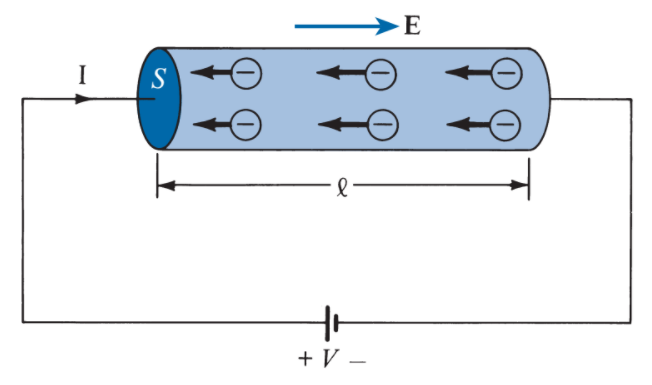
\includegraphics[scale=0.5]{CamposMag/CM21.png}
\caption{Un conductor de sección uniforme de cruce bajo un campo E aplicado.}
\label{fig:conducor bajo campo uniforme}
\end{figure}
El campo eléctrico aplicado es uniforme y su magnitud esta dado por:
\begin{equation}\label{eq:conductor campo}
E=\frac{V}{\textit{l}}
\end{equation}
Dado que el conductor tiene una sección transversal uniforme:
\begin{equation}\label{eq:conductor flujo}
J=\frac{I}{S}
\end{equation}
Usando las ecuaciones \ref{eq:JsigmaE}, \ref{eq:conductor campo} y \ref{eq:conductor flujo}:
\begin{equation}
\frac{I}{S}=\sigma E=\frac{\sigma V}{\textit{l}}
\end{equation}
Acomodando las ecuaciones:
\begin{equation}\label{eq:resistencia}
R=\frac{V}{I}=\frac{\textit{l}}{\sigma S}=\frac{\rho_c\textit{l}}{S}
\end{equation}
Donde:
\begin{itemize}
\item $\rho_c=1\sigma$: es la resistividad del material.
\end{itemize}
\begin{remark}
La ecuación \ref{eq:resistencia} es útil para determinar la resistencia de cualquier conductor de sección transversal uniforme. Si la sección transversal del conductor no es uniforme la ec. \ref{eq:resistencia} no es aplicable.
\end{remark}
Para la resistencia de un conductor no uniforme se sección de cruce:
\begin{equation}
R=\frac{V}{I}=\frac{\int_LE\cdot dl}{\int_S\sigma E\cdot dS}
\end{equation}
La potencia(en \textbf{watts}) se define como la tasa de cambio de energía W (en julios) o fuerza
veces la velocidad.
\begin{equation}
\label{eq:potencia}
P=\int_vE\cdot Jdv
\end{equation}
que es conocida como la ley de Joule. La \textbf{Densidad de potencia} \textit{$w_p$}(W/$m^3$) esta dado por el integrando de la ecuación \ref{eq:potencia}:
\begin{equation}
w_p=\frac{dP}{dv}=E\cdot J=\sigma|E|^2
\end{equation}
Para un conductor con sección transversal uniforme, dv=dS dl, por lo que la ec. \ref{eq:potencia} se convierte en:
\begin{equation}
P=\int_LEdl\int_SJdS=VI=I^2R
\end{equation}
\subsection{Polarización de un dipolo}
Para comprender el efecto macroscópico de un campo eléctrico sobre un dieléctrico, considere un átomo del dieléctrico que consta de una carga negativa -Q (nube de electrones) y una carga positiva +Q (núcleo) como en la Figura \ref{fig: dipolos nubes}. Se puede adoptar una imagen similar para un molécula dieléctrica; podemos tratar los núcleos de las moléculas como cargas puntuales y la estructura electrónica como una sola nube de carga negativa. Como tenemos cantidades iguales de valores positivos y negativos, todo el átomo o molécula es eléctricamente neutro. Cuando un campo eléctrico \textbf{E} se aplica, la carga positiva se desplaza de su posición de equilibrio en la dirección de \textbf{E} por la fuerza $F_+$=Q\textbf{E}, mientras que la carga negativa se desplaza en la dirección opuesta por la fuerza $F_-$=Q\textbf{E}. Un dipolo resulta del desplazamiento de las cargas, y se dice que el dieléctrico está polarizado. En el estado polarizado, la nube de electrones está distorsionada por el campo eléctrico aplicado \textbf{E}. Esta distribución de carga distorsionada es equivalente, por el principio de superposición, a la distribución original más un dipolo cuyo momento es:
\begin{equation}
\label{eq:momento dipolo}
\textbf{p}=Q\textbf{d}
\end{equation}
Donde \textbf{d} es la distancia vectorial desde -Q y +Q como se muestra en la figura \ref{fig:dipolos nubes}. Si existen N dipolos en un volumen $\delta$\textit{v} de un dieléctrico, el momento total de un dipolo debido a un campo eléctrico es:
\begin{equation}
\label{eq:momento N dipolo}
Q_1d_1+Q_2d_2+\ldots +Q_Nd_N = \sum_{k=1}^NQ_kd_k
\end{equation}
Como medida de la intensidad de la polarización, definimos la polarización P (en coulombios por
metro cuadrado) como el momento dipolar por unidad de volumen del dieléctrico; es decir:
\begin{equation}
\label{eq:momento dipolar}
\textbf{P}=\lim_{\delta v\to 0}\frac{\sum_{k=1}^NQ_kd_k}{\delta v}
\end{equation}
\begin{figure}[H]
\centering
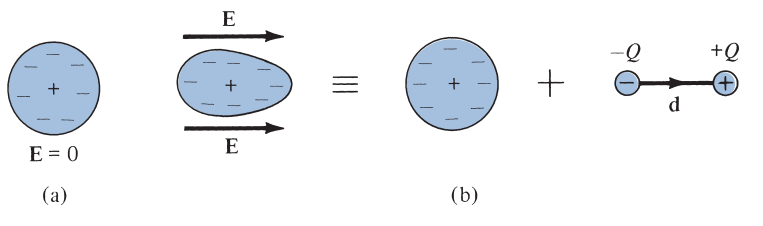
\includegraphics[scale=0.5]{CamposMag/CM22.png}
\caption{Polarización de un átomo o molécula no polarizada.}
\label{fig:dipolos nubes}
\end{figure}

%----------------------------------------------------------------------------------------
\end{document}
